\documentclass[preprint,12pt]{elsarticle}

\usepackage[T1]{fontenc}
\input{glyphtounicode}
\pdfgentounicode=1
\usepackage{amsmath}
\usepackage{amssymb}
\usepackage{booktabs}
\usepackage{graphicx}
\usepackage{url}
\usepackage{xcolor}
\usepackage{algorithm}
\usepackage{algpseudocode}
\usepackage{makecell}

\journal{Robotics and Autonomous Systems}

\begin{document}

\begin{frontmatter}

\title{Query-to-Grasp: A Target-Source Diagnostic Framework for Open-Vocabulary RGB-D Manipulation}

\author[chalmers]{Zhuo Chen\corref{cor1}}
\ead{zhuoc@chalmers.se}
\cortext[cor1]{Corresponding author}
\affiliation[chalmers]{
  organization={Chalmers University of Technology},
  city={Gothenburg},
  country={Sweden}
}

\begin{abstract}
Open-vocabulary detectors can localize language-described objects in 2D, but
robot manipulation requires a geometrically stable, cross-view consistent, and
executable 3D action target. This paper presents Query-to-Grasp, a simulated
diagnostic framework for studying this retrieval-to-execution gap in
language-conditioned RGB-D manipulation. The framework keeps semantic
retrieval, RGB-D lifting, camera-frame alignment, target-source selection,
multi-view memory, re-observation, and scripted execution as separable modules.
This decomposition enables controlled evaluation of which target sources become
executable, rather than treating final task success as a single opaque score.
Across PickCube and StackCube diagnostics, we find that semantic reranking is
not the dominant bottleneck in low-candidate scenes, camera-frame alignment is
necessary for meaningful multi-view memory, crop-level and memory-based target
sources are far more executable than box-center depth, and centimeter-level
target perturbations can sharply reduce pick and place success. A synthetic
RGB-D stress test shows that crop-top-surface targets remain stable under
moderate depth noise and dropout, while box-center depth remains weak. A
500-seed StackCube non-oracle reference-object bridge achieves roughly
45--55\% task success across single-view, tabletop, and closed-loop settings,
while oracle rows remain privileged diagnostic upper bounds. A 1,600-seed
non-cube PickSingleYCB diagnostic shows a large oracle--crop gap: the
privileged oracle target is partially executable, whereas crop-derived targets
remain near failure under the same scripted primitive. The
result is a reproducible simulated benchmark for diagnosing how open-vocabulary
RGB-D retrieval becomes, or fails to become, executable manipulation.
\end{abstract}

%% Research highlights
\begin{highlights}
\item Diagnoses open-vocabulary RGB-D target sources for manipulation.
\item Separates semantic retrieval from executable 3D action targets.
\item Tests target sources under moderate synthetic RGB-D stress.
\item Links centimeter-level target error to execution collapse.
\item Adds a 1,600-seed non-cube PickSingleYCB diagnostic.
\end{highlights}

\begin{keyword}
Open-vocabulary manipulation \sep RGB-D perception \sep Target-source diagnosis
\sep Diagnostic evaluation
\end{keyword}

\end{frontmatter}

\section{Introduction}

Open-vocabulary visual detectors have made it practical to query a robot scene
with natural language and obtain candidate object regions. However, a detected
2D region is not yet a manipulation command. A robot controller needs a 3D
target that is geometrically precise, stable under viewpoint changes, and
compatible with the motion primitive that will execute it. Query-to-Grasp
studies this interface explicitly. We call the 3D quantity passed from
perception to control a \emph{target source}: for example a semantic object
center, a refined crop grasp point, a fused memory grasp target, a predicted
reference-object placement target, or a privileged oracle pose.

We intentionally fix the control layer and study the retrieval-to-execution
interface under controlled simulated conditions. This design isolates
target-source quality before adding policy capacity, learned grasp synthesis,
or physical robot deployment. The central hypothesis is that many
language-conditioned manipulation failures are not purely semantic: they arise
when correct or nearly correct 2D evidence is converted into an unstable,
biased, or controller-incompatible 3D action target.

The study is organized around seven research questions:

\begin{description}
\item[RQ1] Is semantic reranking the main bottleneck?
\item[RQ2] Does camera-frame alignment enable meaningful multi-view memory?
\item[RQ3] Which 3D target sources are executable?
\item[RQ4] What does StackCube reveal beyond PickCube?
\item[RQ5] How sensitive is execution to centimeter-level target error?
\item[RQ6] When is target-source quality insufficient?
\item[RQ7] Do target-source conclusions persist under synthetic RGB-D degradation?
\end{description}

The contributions are:

\begin{itemize}
\item A target-source diagnostic ladder for open-vocabulary RGB-D manipulation,
distinguishing semantic centers, crop baselines, refined grasp points, memory
targets, predicted reference targets, and privileged oracle probes.
\item A modular simulated framework that separates grounding, lifting,
camera-frame alignment, multi-view memory, re-observation, target selection,
and scripted execution.
\item A controlled analysis showing that target-source choice and
centimeter-scale geometric errors strongly shape execution outcomes in the
evaluated settings.
\item A synthetic RGB-D sensor-stress study quantifying how depth noise and
depth dropout affect target-source executability under controlled simulation.
\item A conservative non-cube diagnostic showing that target-source quality and
controller compatibility remain coupled beyond cube geometry.
\end{itemize}

\begin{figure}[t]
\centering
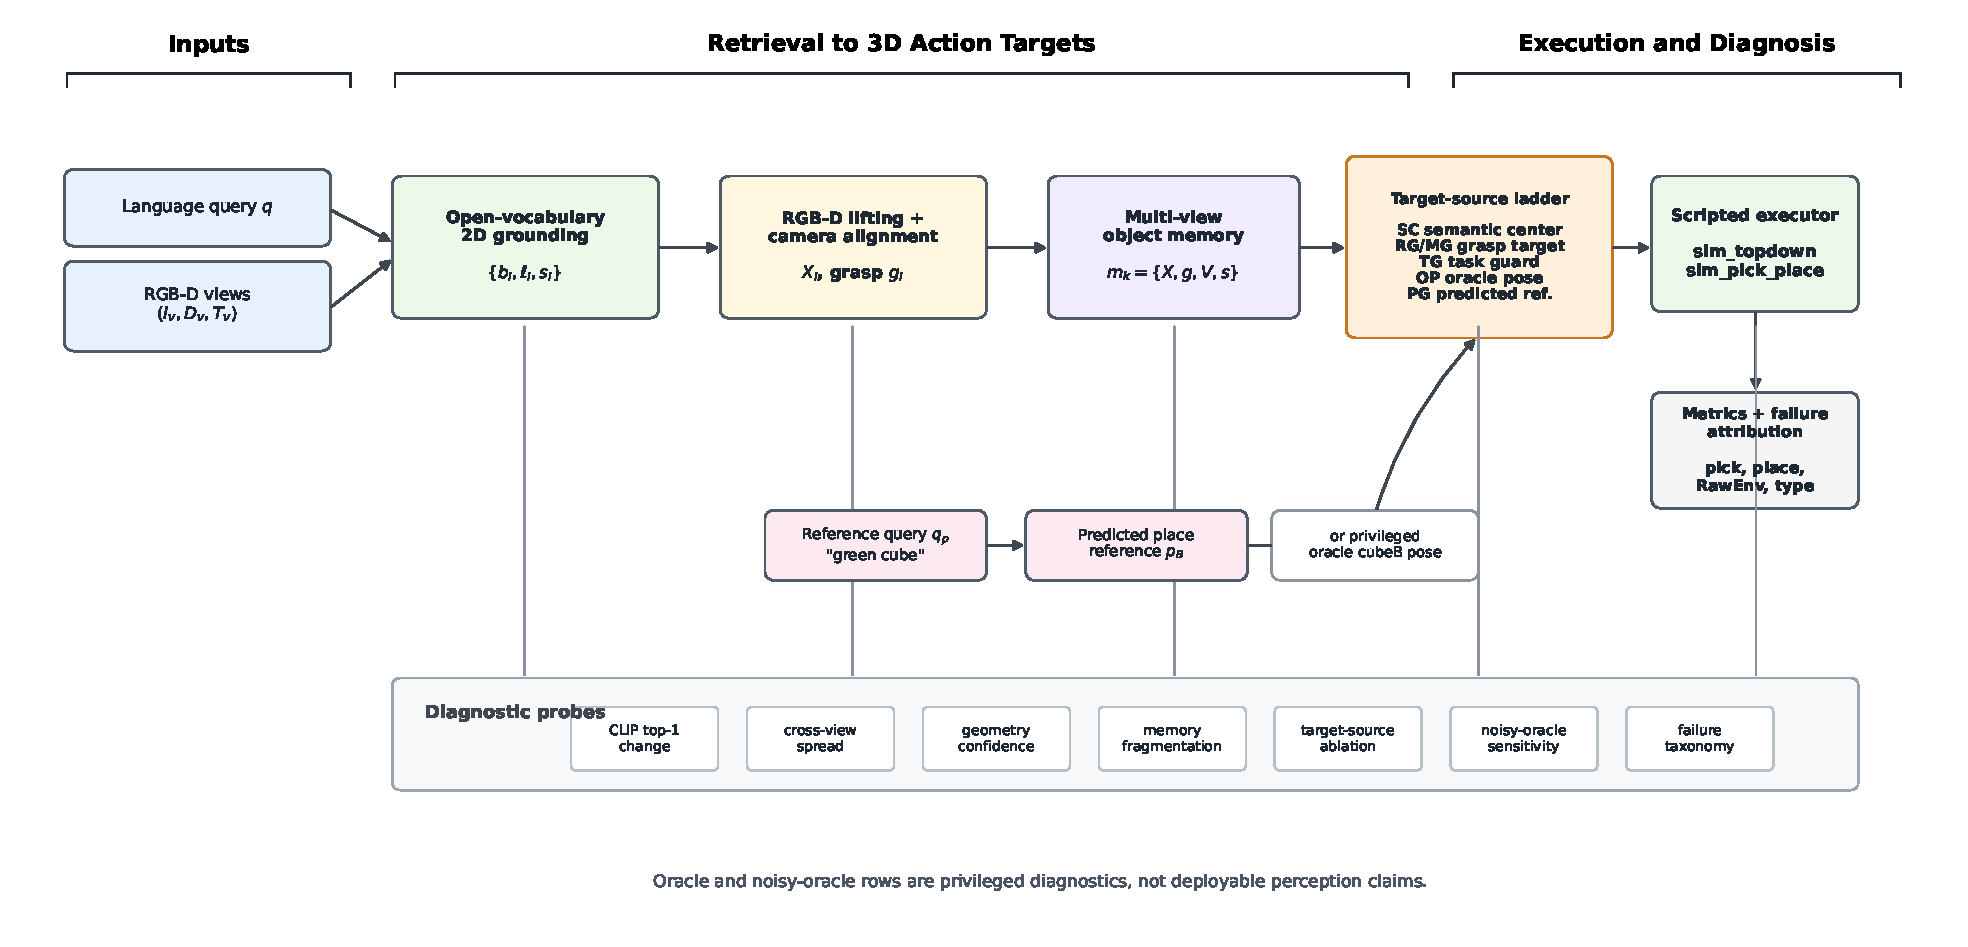
\includegraphics[width=\linewidth]{figures/pipeline_overview_vector.pdf}
\caption{Reproducible variable-flow diagram for Query-to-Grasp. The framework
keeps semantic retrieval, RGB-D lifting, target-source selection, memory,
scripted execution, and failure attribution separable so that each stage can be
diagnosed independently.}
\label{fig:ras-pipeline}
\end{figure}

\section{Related Work}

\subsection{Open-Vocabulary 2D and 3D Grounding}

Open-vocabulary detectors and vision-language models provide reusable
perception primitives for robotics. CLIP aligns image and text representations
and is widely used as a retrieval or scoring component in open-vocabulary
systems~\cite{radford2021learning}. GroundingDINO extends this idea to
language-conditioned object detection by producing boxes and phrases for
open-set prompts~\cite{liu2023groundingdino}. Beyond 2D detection, recent
systems embed language-aligned features into 3D maps, point clouds, or radiance
fields, including OpenScene~\cite{peng2023openscene},
ConceptFusion~\cite{jatavallabhula2023conceptfusion},
CLIP-Fields~\cite{shafiullah2023clipfields}, and
LERF~\cite{kerr2023lerf}. These methods improve semantic access to scenes, but
they do not by themselves evaluate whether a language-indexed 3D region has
become an executable action target for a particular controller. Query-to-Grasp
uses open-vocabulary retrieval as an input and diagnoses the downstream
target-source interface: how the retrieved object becomes a geometrically
stable and executable 3D action target.

\subsection{Language-Conditioned Manipulation}

Language-conditioned manipulation systems often combine semantic perception,
planning, and policy execution. CLIPort couples language-conditioned perception
with manipulation affordances~\cite{shridhar2022cliport}; PerAct uses a
transformer policy over multi-view observations~\cite{shridhar2022peract};
SayCan grounds language-model plans in affordance values~\cite{ahn2022saycan};
and VIMA studies multimodal prompting for robot manipulation~\cite{jiang2023vima}.
Large-scale robot learning systems such as RT-1 and RT-2 further connect
vision-language representations with action prediction~\cite{brohan2022rt1,
brohan2023rt2}. These systems optimize broad task execution, whereas
Query-to-Grasp is narrower and diagnostic. It does not train a policy or claim
general manipulation competence; it asks whether a language-conditioned
retrieval result has become an executable 3D target before policy capacity is
added.

\subsection{RGB-D Grasp Detection and Grasp Pose Generation}

RGB-D grasp detection and 6-DoF grasp synthesis methods estimate graspable
poses from point clouds or depth images. Classical and learning-based grasp
detectors include GPD~\cite{tenpas2017gpd}, Dex-Net/GQ-CNN-style analytic and
synthetic-data grasp learning~\cite{mahler2017dexnet}, Contact-GraspNet for
6-DoF grasp proposal generation~\cite{sundermeyer2021contactgraspnet},
GraspNet-1Billion as a large-scale grasping benchmark~\cite{fang2023graspnet},
and AnyGrasp as a robust grasp-perception system~\cite{fang2023anygrasp}. Such
methods are natural future bridges for Query-to-Grasp. In this paper, however,
we intentionally fix a scripted executor and compare deterministic target
sources. The external crop baselines answer a focused diagnostic question:
after an open-vocabulary detector selects an object crop, is a box center depth
point enough, or does execution require stronger RGB-D geometry?

\subsection{Multi-View Memory and Active Perception}

Multi-view object memory and active perception can improve recall, reduce
occlusion, and resolve semantic uncertainty. However, additional views also
create calibration, association, and fusion problems. Query-to-Grasp treats
multi-view memory and re-observation as separable diagnostic modules. The
important metric is not only whether uncertainty decreases, but whether the
final target source remains executable by the fixed controller. This distinction
matters because a fused object hypothesis can have more semantic support while
also drifting geometrically or absorbing observations from the wrong object.

\subsection{Benchmarks and Diagnostic Evaluation}

Robotic manipulation benchmarks such as RLBench, Meta-World, CALVIN, and
ManiSkill provide reproducible tasks, standardized success signals, and
increasingly diverse language or manipulation settings~\cite{james2020rlbench,
yu2020metaworld, mees2022calvin, gu2023maniskill2}. Final task success is
essential, but it can hide the source of failure in language-conditioned
systems. A robot may fail because retrieval selected the wrong object, RGB-D
lifting produced a biased target, multi-view memory merged inconsistent
observations, or the controller was geometrically incompatible with the target.
Query-to-Grasp complements task benchmarks by turning these interfaces into
explicit diagnostic variables.

\section{Problem Formulation}

Let a language query be denoted by $q$, an RGB-D observation by $(I, D)$, a 2D
proposal by $b$, camera intrinsics by $K$, and the camera-to-world transform by
$T_{wc}$. A target source $s$ maps the detected evidence to a 3D action target
$p_s \in \mathbb{R}^3$. An executor $E$ attempts to act on $p_s$ and produces
outcomes
\[
  y = \{\text{target\_available}, \text{pick\_success},
  \text{place\_success}, \text{task\_success}\}.
\]

The diagnostic question is:
\[
  \text{Given } (q, I, D, b, K, T_{wc}), \text{ which } p_s
  \text{ is executable, and where do failures enter?}
\]

This formulation separates semantic retrieval from target-source quality. A
detector may correctly identify the target object while the selected 3D point
remains too noisy, too biased, poorly fused across views, or incompatible with
the controller.

For a pixel $u=(u_x,u_y)$ with depth $d(u)$, the lifted camera-frame point is
\[
  x_c(u) = d(u)K^{-1}[u_x, u_y, 1]^\top ,
\]
and the world-frame point is
\[
  x_w(u) = T_{wc} \begin{bmatrix} x_c(u) \\ 1 \end{bmatrix}.
\]
Different target sources choose different subsets or summaries of the lifted
points inside a language-conditioned proposal. A semantic center may use the
median or centroid of crop points, a crop top-surface source may filter for
elevated object support, a memory target may aggregate observations across
views, and an oracle target may use simulator state. The diagnostic ladder
therefore compares maps
\[
  f_s(q, I, D, b, K, T_{wc}) \rightarrow p_s
\]
under the same executor whenever possible.

The metrics are deliberately separated. \texttt{target\_available} measures
whether a 3D target source was formed. \texttt{pick\_success} measures whether
the object was grasped or lifted according to ManiSkill evidence.
\texttt{place\_success} measures whether a StackCube placement was confirmed.
\texttt{task\_success} is the environment's raw task flag for pick-place rows.
For pick-only rows, raw environment success is reported only as a diagnostic
flag and is not the primary metric.

\section{Method}

\subsection{Query-Conditioned 2D Grounding}

The system receives a query and one or more RGB-D views. GroundingDINO returns
2D boxes, phrases, and confidence scores. Optional CLIP reranking can rescore
the candidate list. In the evaluated low-candidate scenes, reranking did not
change the top-1 candidate, which motivates the paper's emphasis on downstream
geometry.

The detector output for a view $v$ is a set of candidates
$\{(b_i, c_i, \ell_i)\}$ with boxes $b_i$, detector confidences $c_i$, and
phrases or labels $\ell_i$. If CLIP reranking is enabled, crops are scored
against the query and the candidate order can be updated. The benchmark logs
both the number of detector candidates and whether the top-1 candidate changes
after reranking. This makes semantic reranking a measured variable rather than
an assumed improvement.

\subsection{RGB-D Lifting and Camera-Frame Alignment}

Valid depth pixels are lifted through the camera model and transformed to world
coordinates using $T_{wc}$. Camera-frame alignment is evaluated separately
because multi-view memory is meaningful only if observations from different
views occupy a common frame.

For crop-based sources, valid depth pixels are restricted to the selected 2D
box before workspace filtering. The implemented workspace filter keeps points
near the tabletop interaction region: $|x|, |y| \leq 0.20$ m and
$z \in [-0.02, 0.08]$ m in the world frame, with at least 20 workspace points.
The refined and crop-top-surface sources estimate support height from the
10th-percentile $z$ value, keep elevated points at least 0.015 m above that
support, require at least 12 elevated points when possible, cluster the
elevated XY points with a 0.03 m radius, and choose the largest low-spread
component. The final target uses the component median XY and a local support
height estimated within a 0.04 m radius and 0.012 m support margin, with
workspace-median fallbacks when elevated support is insufficient. This is
intentionally deterministic: it tests how far a standard RGB-D crop heuristic
can go without a learned grasp network.

\subsection{Target-Source Ladder}

The target-source ladder contains both deployable and privileged sources:

\begin{itemize}
\item SC: semantic center.
\item RG: refined grasp point.
\item MG: memory grasp target.
\item TG: task-guarded target.
\item PG/PB: predicted green or broad reference target.
\item OA/OB: privileged oracle cubeA or cubeB pose.
\item Crop baselines: box center depth, crop median, crop top-surface.
\item Oracle object pose: privileged upper bound.
\end{itemize}

\begin{table}[t]
\centering
\caption{Target-source ladder used by the RAS manuscript. Privileged sources
are diagnostic probes and are not deployable perception claims.}
\label{tab:ras-target-sources}
\begin{tabular}{lll}
\toprule
Code & Source & Diagnostic role \\
\midrule
SC & semantic center & raw RGB-D object center \\
RG & refined grasp & local crop geometry target \\
MG & memory grasp & multi-view fused grasp target \\
TG & task guarded & task-aware selected object target \\
BC & box center depth & simplest crop baseline \\
CM & crop median & crop aggregation baseline \\
CT & crop top-surface & deterministic crop heuristic \\
PG/PB & predicted reference & explicit/broad place target \\
OA/OB & oracle pose & privileged upper bound \\
\bottomrule
\end{tabular}
\end{table}

\subsection{Multi-View Memory}

Object memory merges compatible detections across views and stores labels,
scores, view support, lifted points, and grasp-target observations. The current
implementation uses a merge radius of 0.08 m and merges only compatible labels
or parsed attributes. Fused grasp targets are represented by robust aggregate
geometry rather than a single detected pixel.

Compatibility is conservative: detections are candidates for merging when their
normalized labels or parsed attributes agree and their 3D centers fall within
the merge radius. Color or category conflicts are not merged. Memory objects
store support views, confidence summaries, geometry confidence, and grasp
observations. For memory grasp targets, the selected target is a robust
aggregate over supported grasp observations rather than a single view's raw
semantic center. This is the mechanism evaluated in the PickCube memory result.

\subsection{Re-Observation}

Re-observation is triggered when support or confidence is insufficient:
\[
v < 2 \quad \lor \quad \Delta c < \tau_{\mathrm{gap}} \quad \lor \quad
c < \tau_{\mathrm{conf}} \quad \lor \quad
g < \tau_{\mathrm{geo}} \quad \lor \quad n < \tau_{\mathrm{pts}}.
\]
The current thresholds are $\tau_{\mathrm{gap}}=0.05$,
$\tau_{\mathrm{conf}}=0.50$, $\tau_{\mathrm{geo}}=0.50$, and
$\tau_{\mathrm{pts}}=100$. The closed-loop result is interpreted
diagnostically, not as a blanket claim that more views improve execution.

\subsection{Scripted Executors}

The fixed executors are diagnostic instruments. \texttt{sim\_topdown} tests
whether a selected pick target is already executable by a top-down primitive.
\texttt{sim\_pick\_place} extends this to a scripted placement probe. These
controllers are intentionally held fixed so that changes in success can be
attributed to target-source quality, target association, and placement
precision.

For reproducibility, the default top-down pick executor moves the end effector
to \(0.12\,\mathrm{m}\) above the selected target, descends to a grasp height of
\(z+0.025\,\mathrm{m}\), closes the gripper, and lifts to \(z+0.18\,\mathrm{m}\).
The fixed stage budget is 40/30/20/40 simulation steps for move, descend,
close, and lift. The pick-place executor uses the same pick primitive and then
moves \(0.12\,\mathrm{m}\) above the selected place target, descends for 30
steps, opens for 20 steps, and settles for 20 steps. The action convention is a
Cartesian end-effector delta plus gripper command, with the same constants used
for all target sources in a comparison.

\begin{algorithm}[t]
\caption{Query-to-Grasp target selection and diagnostic execution}
\label{alg:query-to-grasp}
\begin{algorithmic}[1]
\Require Query $q$, RGB-D views $\{(I_v,D_v,K_v,T_{wc,v})\}$, target-source mode $s$
\State Parse $q$ into grounding prompt and optional reference query.
\For{each view $v$}
  \State Detect candidate boxes and phrases with GroundingDINO.
  \State Optionally rerank crops with CLIP and log top-1 changes.
  \State Lift valid crop depth pixels to world points.
  \State Compute single-view target candidates for the requested source $s$.
\EndFor
\State Merge compatible detections into multi-view object memory.
\If{re-observation trigger is active}
  \State Acquire diagnostic view(s), update memory, and log trigger reasons.
\EndIf
\State Select pick target from SC/RG/MG/TG/crop/oracle source.
\If{pick-place task}
  \State Select place target from predicted reference or oracle source.
\EndIf
\State Execute with fixed scripted controller.
\State Record target availability, pick, place, task, and failure type.
\end{algorithmic}
\end{algorithm}

\section{Experimental Design}

Table~\ref{tab:experiment-map} summarizes the main RAS evidence map.

\begin{table}[t]
\centering
\caption{RAS experiment map. Oracle rows are privileged diagnostics, not
deployable perception claims.}
\label{tab:experiment-map}
\begin{tabular}{llll}
\toprule
RQ & Evidence & Primary metric & Claim boundary \\
\midrule
RQ1 & CLIP ablation & top-1 change, pick & low-candidate scenes \\
RQ2 & camera alignment & spread, fragmentation & simulation camera frames \\
RQ3 & crop/source ladder & pick/task success & scripted executor \\
RQ4 & StackCube bridge & task success & explicit reference query \\
RQ5 & noisy oracle + target-error bins & pick/place/task & sensitivity probe \\
RQ6 & non-cube aggregate & pick success & controller mismatch \\
RQ7 & synthetic RGB-D stress & pick/task success & simulation proxy \\
\bottomrule
\end{tabular}
\end{table}

All experiments are simulated ManiSkill diagnostics. The executor, detector,
and target-source definitions are held fixed within each comparison so that
the measured variable is the source of the 3D action target. For pick-only
experiments, the primary metric is \texttt{pick\_success}; the environment's
raw task flag is logged but not interpreted as task completion. For StackCube
pick-place experiments, the primary metric is \texttt{task\_success}, with
\texttt{pick\_success} and \texttt{place\_success} retained for failure
attribution. Oracle rows use privileged simulator state and are included only
as diagnostic upper bounds.

\section{Results}

\subsection{RQ1: Is Semantic Reranking the Main Bottleneck?}

In the current low-candidate scenes, CLIP reranking did not change the top-1
candidate for either PickCube or StackCube. PickCube reached 50/50 pick success
with zero top-1 changes and StackCube reached 44/50 pick success with zero
top-1 changes. This does not imply that CLIP is generally unimportant; it means
that these failures are better explained by the 3D target source than by
semantic candidate ranking.

This result fixes the scope of the paper. In high-clutter or high-ambiguity
settings, semantic reranking may become important. In the present benchmark,
however, the average number of detections is low: 1.04 on PickCube and 1.48 on
StackCube. The system therefore has little semantic ranking work to do. The
remaining failures occur after top-1 selection, when the selected crop must be
converted into an executable 3D target. This motivates the subsequent
target-source experiments.

\subsection{RQ2: Does Camera-Frame Alignment Enable Multi-View Memory?}

Camera-frame alignment reduces cross-view spread from 1.0693 m to 0.0518 m and
memory fragmentation from 3.3333 to 1.3333 objects/run. This result supports
the claim that multi-view memory is a geometric system component, not simply a
collection of more detections.

The magnitude of this change matters for manipulation. A one-meter cross-view
spread makes object memory meaningless for tabletop execution; the memory is
effectively storing incompatible coordinate frames. After correction, the
remaining spread is on the order of centimeters, which is still relevant for
grasping but small enough to support object-level fusion. This is why camera
alignment is presented before the manipulation tables: without a common frame,
multi-view confidence and support-view counts cannot be interpreted as reliable
action evidence.

\begin{figure}[t]
\centering
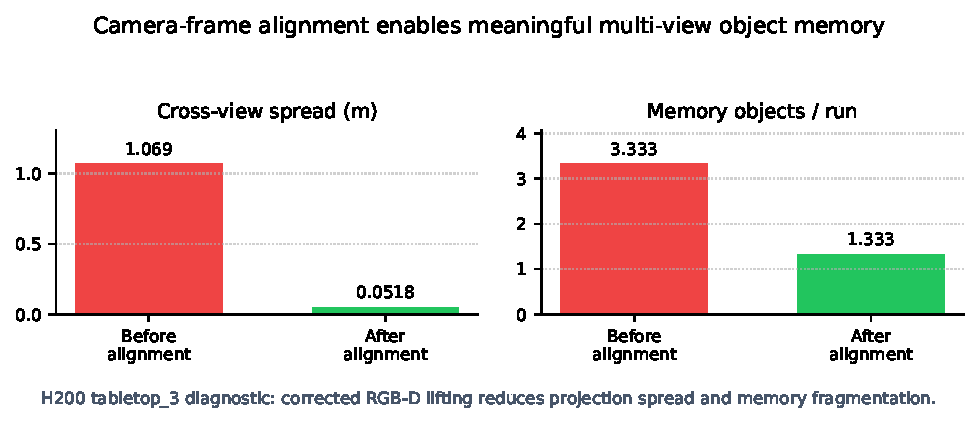
\includegraphics[width=0.9\linewidth]{figures/geometry_memory_ablation.pdf}
\caption{Camera-frame alignment reduces cross-view spread and memory
fragmentation.}
\label{fig:ras-geometry-memory}
\end{figure}

\subsection{RQ3: Which 3D Target Sources Are Executable?}

The external RGB-D crop baseline shows that a 2D box center is a poor action
target, while crop aggregation and top-surface filtering are strong clean-scene
baselines.

\begin{figure}[t]
\centering

\includegraphics[width=\linewidth]{figures/ras_crop_baseline_ci.pdf}
\caption{External RGB-D crop baselines with Wilson 95\% confidence intervals.
Additional held-out seeds extend the main comparable rows to 400 runs; rows
with fewer matched artifacts keep their actual $N$. Pick-only groups use pick
success; StackCube pick-place uses task success with a predicted reference
target.}
\label{fig:ras-crop-ci}
\end{figure}

\begin{table}[t]
\centering
\caption{External RGB-D crop baselines. The success column reports the primary
metric with Wilson 95\% confidence intervals and each row keeps its actual
number of completed runs.}
\label{tab:ras-external-crop}
\resizebox{\linewidth}{!}{%
\input{tables/table_external_crop_with_ci.tex}
}
\end{table}

The gap between \texttt{box\_center\_depth} and crop-level sources is the
clearest target-source result. On PickCube, a single lifted box-center depth
point reaches only 0.010 pick success, while \texttt{crop\_median} reaches
0.925 and \texttt{crop\_top\_surface} reaches 0.980 over 400 runs. On
StackCube pick-only, box-center depth reaches 0.060, while crop aggregation
reaches about 0.78 over 400 runs.
Thus the open-vocabulary detector has already done enough semantic work to
select the object, but the simplest possible 3D point source is not an
actionable grasp target. The crop baselines should not be read as competitors
to a learned grasp generator; they are additional rungs in the diagnostic
ladder.

\subsection{RQ4: What Does StackCube Reveal Beyond PickCube?}

StackCube exposes placement-target and reference-object limitations that do not
appear in PickCube. The non-oracle explicit green-cube reference bridge reaches
0.552, 0.472, and 0.446 task success over 500 seeds in single-view, tabletop,
and closed-loop modes. The broad reference query is weaker, reaching 0.360 in
single-view over 200 seeds. Oracle pick-place reaches 0.880 task success and is
reported only as a privileged upper bound.

The StackCube result is intentionally not framed as solved stacking. Instead,
it decomposes the task into target-source questions. Pick-only rows ask whether
the query-derived cubeA target can support grasping. Predicted-place rows ask
whether an explicit reference-object query, such as the green cube, can provide
a non-oracle placement destination. Broad-reference rows ask whether a less
specific query, such as ``cube'', is sufficient. Oracle rows ask how much
success remains possible when both pick and place targets are privileged. The
gap between predicted-place and oracle rows therefore measures placement-target
and reference-association limits, not only controller limits.

The saved per-run artifacts also allow a focused placement-target error view
for the subset of StackCube rows with matched oracle cubeB targets. Across
1,412 rows, place/task success remains around 0.60 for sub-centimeter
placement errors, drops to 0.240 for 2--5 cm errors, and is essentially zero
above 5 cm. This analysis does not cover every predicted-place seed because
some rows lack a same-seed oracle place artifact, but it directly supports the
claim that StackCube failures are strongly shaped by placement-target
precision.

\begin{figure}[t]
\centering
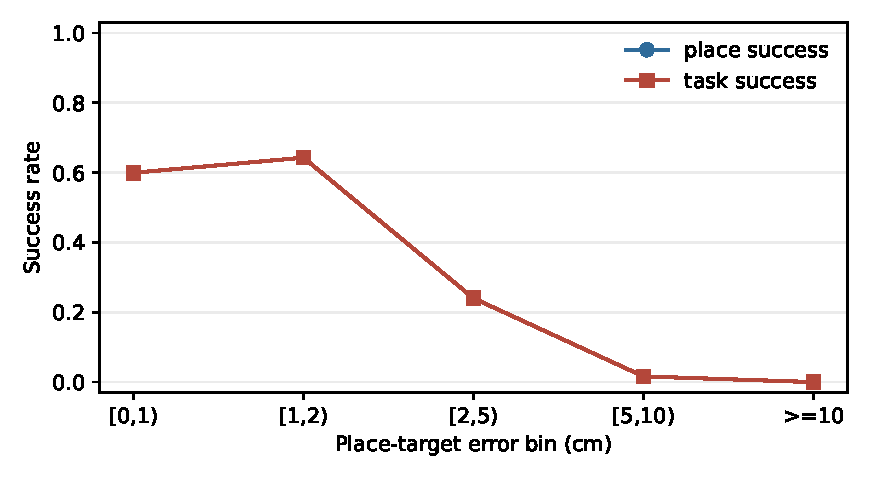
\includegraphics[width=\linewidth]{figures/figure_place_error_success.pdf}
\caption{StackCube place-target error diagnostic for rows with matched oracle
cubeB targets. Place and task success decrease sharply once placement error
enters the multi-centimeter range.}
\label{fig:place-error-success}
\end{figure}

\begin{table}[t]
\centering
\caption{StackCube place-target error bins. This derived analysis uses only
rows with matched oracle cubeB place targets.}
\label{tab:place-error-bins}
\resizebox{\linewidth}{!}{%
\begin{tabular}{lrrr}
\toprule
Place error (cm) & N & Place success & Task success \\
\midrule
\mbox{[0,1)} & 754 & 0.599 & 0.599 \\
\mbox{[1,2)} & 126 & 0.643 & 0.643 \\
\mbox{[2,5)} & 283 & 0.240 & 0.240 \\
\mbox{[5,10)} & 184 & 0.016 & 0.016 \\
\mbox{$\geq$10} & 65 & 0.000 & 0.000 \\
\bottomrule
\end{tabular}

}
\end{table}

\begin{figure}[t]
\centering

\includegraphics[width=\linewidth]{figures/ras_target_ladder.pdf}
\caption{RAS target-source ladder with Wilson 95\% confidence intervals.
PC denotes PickCube, SC denotes StackCube, and oracle rows are privileged
diagnostic probes.}
\label{fig:ras-target-ladder}
\end{figure}

\begin{table}[t]
\centering
\caption{Target-source ladder used for the RAS result narrative. PC denotes
PickCube, SC denotes StackCube, and PG denotes the predicted green-cube
reference. Oracle rows are privileged diagnostics, not deployable perception
results.}
\label{tab:ras-target-ladder-results}
\resizebox{\linewidth}{!}{%
\begin{tabular}{lllll}
\toprule
Setting & Source & Metric & Success (95\% CI) & Claim \\
\midrule
PC pick & semantic center & pick & 0.964 [0.877, 0.990] & pick ablation \\
PC pick & refined grasp & pick & 1.000 [0.935, 1.000] & pick ablation \\
PC tabletop & memory grasp & pick & 1.000 [0.935, 1.000] & simulated pick \\
PC pick & crop top-surface & pick & 0.980 [0.961, 0.990] & crop diagnostic \\
SC Q+PG single & predicted green ref. & task & 0.552 [0.508, 0.595] & non-oracle bridge \\
SC Q+PG tabletop & predicted green ref. & task & 0.472 [0.429, 0.516] & non-oracle bridge \\
SC Q+PG closed-loop & predicted green ref. & task & 0.446 [0.403, 0.490] & non-oracle bridge \\
SC broad ref. single & predicted broad ref. & task & 0.360 [0.297, 0.429] & query specificity \\
SC oracle pick-place & oracle A + oracle B & task & 0.880 [0.762, 0.944] & oracle upper bound \\
\bottomrule
\end{tabular}

}
\end{table}

\subsection{RQ5: How Sensitive Is Execution to Centimeter-Level Target Error?}

Noisy-oracle perturbations show that small geometric errors can sharply reduce
execution. Pick and place success drop sharply as target perturbation increases
from 1 cm to 5 cm.

The noisy-oracle experiment supplies a mechanism for the previous observations.
If a privileged pick target is perturbed by 2 cm, PickCube pick success drops
to 0.488 and StackCube pick success drops to 0.404 over the combined 250-run
result. At 5 cm, both settings are near failure. For StackCube pick-place, place perturbations are similarly
destructive: with clean pick targets, a 5 cm place perturbation leaves only
0.040 task success over 250 runs. This explains why visually small cross-view or
reference-target errors can determine downstream manipulation outcomes.

We also derive a target-error view from the saved per-run artifacts. For
ordinary target-source rows, each seed is matched to the same-seed
oracle-object row and the Euclidean distance between executed pick targets is
computed. For noisy-oracle rows, the recorded applied perturbation supplies the
error magnitude. This produces 9,369 artifact-backed rows spanning the external
crop baseline, the PickSingleYCB diagnostic, and the noisy-oracle probes. The
trend in Fig.~\ref{fig:target-error-bins} is deliberately not presented as a
predictive model; it is a diagnostic aggregation showing that success remains
high for several sub-centimeter and near-centimeter bins but collapses once
target-source deviations move into the multi-centimeter range. Because the bins
aggregate different tasks and target-source families, the sub-centimeter bins
should not be interpreted as a calibrated monotonic curve. The robust pattern
is the sharp degradation once errors enter the multi-centimeter regime.
Across this aggregation, successful picks have median target error 0.67 cm,
whereas failed picks have median target error 39.69 cm; the large gap is driven
primarily by non-cube crop targets and high-noise probes.

\begin{figure}[t]
\centering
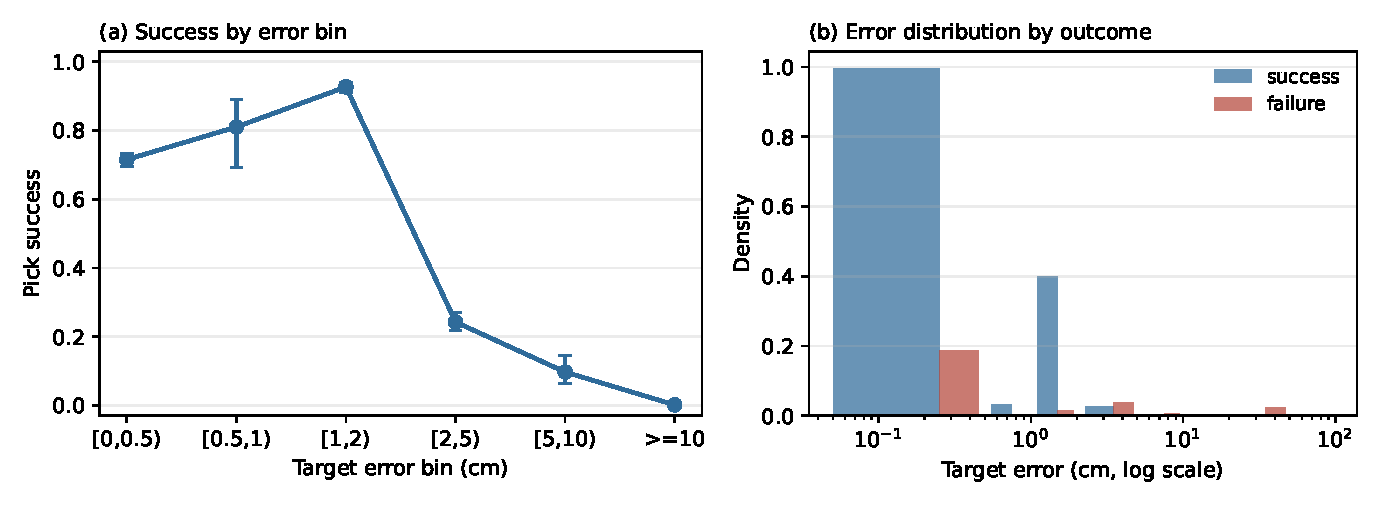
\includegraphics[width=\linewidth]{figures/figure_target_error_mechanism.pdf}
\caption{Target-error diagnostics. (a) Pick success by target-error bin.
(b) Distribution of target error for successful and failed picks. Error is
computed from matched oracle-object targets for real target-source rows and
from recorded perturbations for noisy-oracle rows.}
\label{fig:target-error-bins}
\end{figure}

\begin{table}[t]
\centering
\caption{Target-error bins and pick outcomes. Error is computed from matched
oracle-object targets for real target-source rows and from the recorded
perturbation for noisy-oracle rows.}
\label{tab:target-error-bins}
\resizebox{\linewidth}{!}{%
\begin{tabular}{lrrr}
\hline
Error bin (cm) & N & Pick success & Median error \\
\hline
\mbox{[0,0.5)} & 2091 & 0.715 [0.696,0.734] & 0.00 \\
\mbox{[0.5,1)} & 58 & 0.810 [0.691,0.891] & 0.81 \\
\mbox{[1,2)} & 1300 & 0.927 [0.911,0.940] & 1.71 \\
\mbox{[2,5)} & 985 & 0.243 [0.217,0.270] & 2.62 \\
\mbox{[5,10)} & 196 & 0.097 [0.063,0.146] & 7.42 \\
\mbox{$\geq$10} & 4739 & 0.001 [0.001,0.003] & 41.15 \\
\hline
\end{tabular}

}
\end{table}

\begin{figure}[t]
\centering

\includegraphics[width=\linewidth]{figures/ras_noisy_oracle_sensitivity.pdf}
\caption{Noisy-oracle sensitivity. Perturbing privileged target sources by
centimeter-scale noise sharply reduces pick, place, or task success.}
\label{fig:ras-noisy-oracle}
\end{figure}

\begin{table}[t]
\centering
\caption{Noisy-oracle sensitivity. Rows report the primary metric with Wilson
95\% confidence intervals.}
\label{tab:ras-noisy-oracle}
\resizebox{\linewidth}{!}{%
\begin{tabular}{lllllll}
\toprule
Environment & Mode & Target source & Place source & N & Metric & Success (95\% CI) \\
\midrule
PickCube-v1 & noisy pick & oracle\_object\_pose + 1cm pick noise & none & 250 & pick & 0.824 [0.772, 0.866] \\
PickCube-v1 & noisy pick & oracle\_object\_pose + 2cm pick noise & none & 250 & pick & 0.488 [0.427, 0.550] \\
PickCube-v1 & noisy pick & oracle\_object\_pose + 5cm pick noise & none & 250 & pick & 0.112 [0.079, 0.157] \\
StackCube-v1 & noisy pick & oracle\_object\_pose + 1cm pick noise & none & 250 & pick & 0.740 [0.682, 0.790] \\
StackCube-v1 & noisy pick & oracle\_object\_pose + 2cm pick noise & none & 250 & pick & 0.404 [0.345, 0.466] \\
StackCube-v1 & noisy pick & oracle\_object\_pose + 5cm pick noise & none & 250 & pick & 0.068 [0.043, 0.106] \\
StackCube-v1 & noisy place & oracle\_object\_pose & oracle\_cubeB\_pose + 1cm place noise & 50 & task & 0.520 [0.385, 0.652] \\
StackCube-v1 & noisy place & oracle\_object\_pose & oracle\_cubeB\_pose + 2cm place noise & 250 & task & 0.312 [0.258, 0.372] \\
StackCube-v1 & noisy place & oracle\_object\_pose & oracle\_cubeB\_pose + 5cm place noise & 250 & task & 0.040 [0.022, 0.072] \\
\bottomrule
\end{tabular}

}
\end{table}

\subsection{RQ6: When Is Target-Source Quality Insufficient?}

The non-cube diagnostic separates target-source error from controller
feasibility. With the required YCB assets installed, PickSingleYCB-v1 runs
without child failures over 1,600 matched seeds per target source. A privileged
oracle object pose reaches 0.635 pick success, showing that the scripted
top-down primitive can execute a substantial subset of the non-cube settings.
However, the same seeds with \texttt{box\_center\_depth},
\texttt{crop\_median}, and \texttt{crop\_top\_surface} reach only 0.016,
0.029, and 0.036 pick success, respectively. All four sources form a 3D target
on every run, so the weak crop-derived rows are not detection-availability
failures. They instead expose a target-source gap: the RGB-D crop contains
geometric evidence, but the selected action point is rarely compatible with
the top-down primitive on non-cube object geometry.

This result remains deliberately conservative. It is not a claim of broad YCB
manipulation, learned grasping, or robust object generalization. The earlier
compatibility checks also separate runtime compatibility failures from manipulation
evidence; broken or unregistered environments are not counted as negative manipulation results.
LiftPeg remains informative as an executor-mismatch diagnostic: a long peg is poorly matched to the cube-oriented vertical grasp
primitive even when a target exists. Together, PickSingleYCB and LiftPeg show
that target-source quality is necessary but not sufficient; the selected target
must also be compatible with the grasp or control strategy.

\begin{table}[t]
\centering
\caption{Non-cube PickSingleYCB diagnostic over 1,600 matched seeds per target
source. Oracle rows are
privileged executor-feasibility probes, not deployable perception results.}
\label{tab:ras-noncube-gate}
\resizebox{\linewidth}{!}{%
\begin{tabular}{lrrrrrl}
\toprule
Target source & N & Target & Attempt & Pick & 95\% CI & Boundary \\
\midrule
Box center & 1600 & 1.000 & 1.000 & 0.016 & [0.011, 0.023] & non-cube crop target-source diagnostic \\
Crop median & 1600 & 1.000 & 1.000 & 0.029 & [0.022, 0.039] & non-cube crop target-source diagnostic \\
Crop top-surface & 1600 & 1.000 & 1.000 & 0.036 & [0.028, 0.046] & non-cube crop target-source diagnostic \\
Oracle object pose & 1600 & 1.000 & 1.000 & 0.635 & [0.611, 0.658] & privileged executor-feasibility probe \\
\bottomrule
\end{tabular}

}
\end{table}

\begin{figure}[t]
\centering
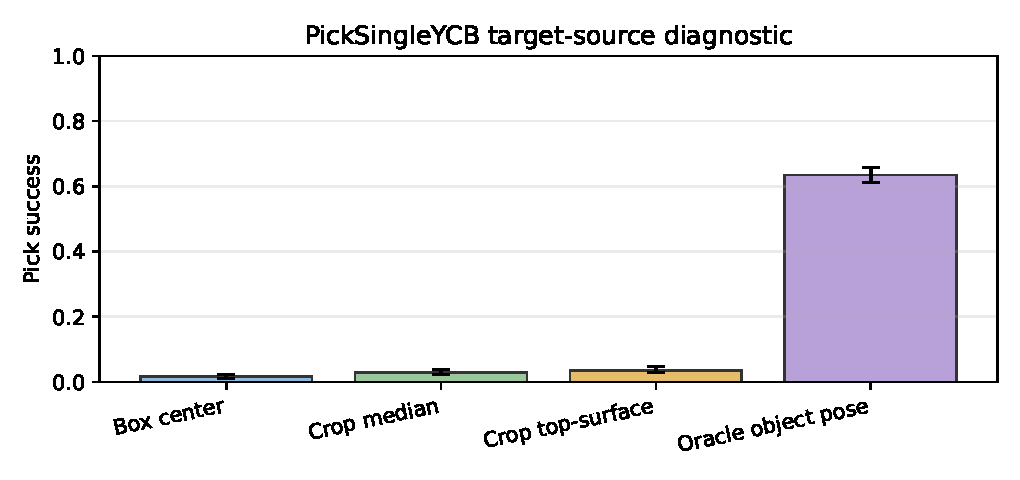
\includegraphics[width=0.8\linewidth]{figures/ras_ycb_noncube_ladder.pdf}
\caption{PickSingleYCB non-cube target-source ladder over 1,600 matched seeds.
The oracle target is partially executable, while crop-derived targets remain
unreliable under the same top-down scripted executor.}
\label{fig:ras-ycb-noncube}
\end{figure}

\begin{figure}[t]
\centering
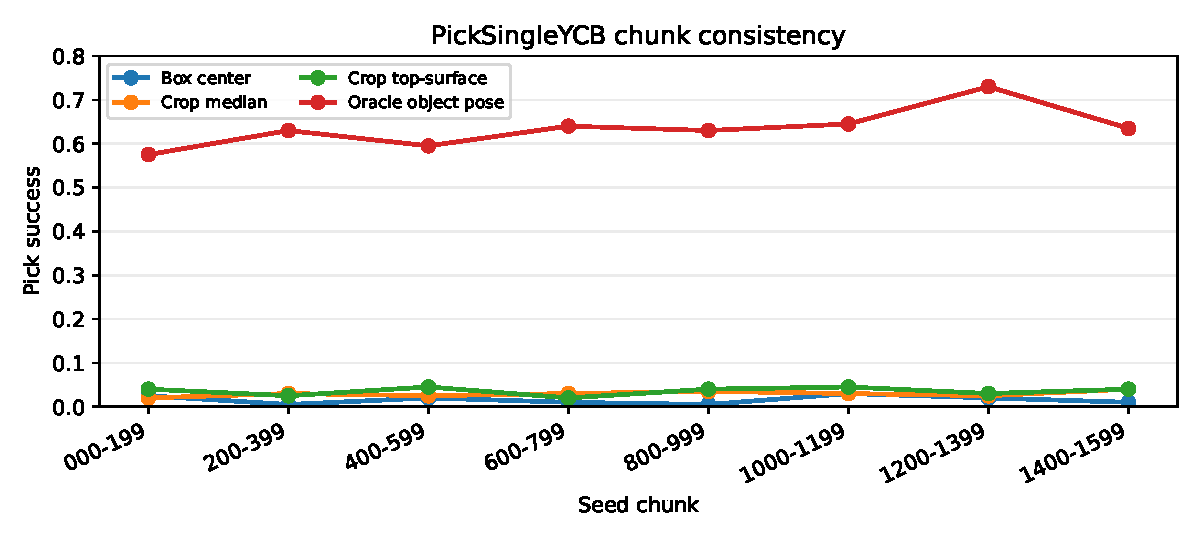
\includegraphics[width=\linewidth]{figures/ras_ycb_chunk_consistency.pdf}
\caption{Chunk consistency for the PickSingleYCB diagnostic. The low
crop-derived pick rates and the much higher oracle pick rate persist across
held-out seed chunks, indicating a systematic target-source gap rather than a
single favorable or unfavorable seed range.}
\label{fig:ras-ycb-chunk-consistency}
\end{figure}

\subsection{RQ7: Do Target-Source Conclusions Persist Under Synthetic RGB-D Degradation?}

The synthetic sensor-stress study tests whether the external crop baseline
result is an artifact of perfectly clean depth. We perturb the depth image
before target extraction with Gaussian depth noise of 5--10 mm or random
valid-depth dropout of 10--20\%, then rerun the same target-source ladder with
matched seeds. This experiment is a simulation proxy for common RGB-D failure
modes, not a replacement for physical RealSense or robot-arm validation.

Table~\ref{tab:sensor-stress-compact} and
Fig.~\ref{fig:sensor-stress-pick} show that
the main target-source conclusion is stable under these moderate perturbations.
The single-pixel \texttt{box\_center\_depth} source remains weak on both
PickCube and StackCube, even when noise occasionally moves the sampled depth
toward a more favorable point. In contrast, \texttt{crop\_top\_surface}
remains near 0.97--1.00 pick success on PickCube and 0.80--0.84 on StackCube
pick-only across all tested noise and dropout levels. The StackCube pick-place
rows show the same pattern at the task level: the predicted-reference bridge
remains around 0.57--0.61 task success under these perturbations
(Fig.~\ref{fig:sensor-stress-task}). Thus, within this controlled range,
target-source choice dominates the tested depth degradation.

This result should be read conservatively. It does not show real-world
robustness, nor does it cover calibration drift, reflective surfaces,
motion blur, relation-heavy clutter, or full sensor failure. Instead, it
adds a reproducible stress-test hook to the diagnostic framework and shows
that the crop-top-surface conclusion is not fragile to modest synthetic depth
noise or dropout in the evaluated cube tasks.

Table~\ref{tab:sensor-stress-compact} summarizes the main stress-test trend;
the full Wilson-interval table is provided in Appendix~\ref{app:sensor-stress}.

\begin{table}[t]
\centering
\caption{Compact synthetic RGB-D sensor-stress summary. Values are success
rates. Pick-only rows report pick success; the StackCube pick-place row reports
task success with crop-top-surface pick targets and predicted green-cube
placement.}
\label{tab:sensor-stress-compact}
\small
\begin{tabular}{llllll}
\toprule
Task / source & Clean & 5mm & 10mm & Drop10 & Drop20 \\
\midrule
PickCube pick / box center & 0.01 & 0.08 & 0.20 & 0.06 & 0.11 \\
PickCube pick / crop top-surface & 0.99 & 1.00 & 0.97 & 0.98 & 0.97 \\
StackCube pick / box center & 0.08 & 0.19 & 0.28 & 0.10 & 0.15 \\
StackCube pick / crop top-surface & 0.84 & 0.80 & 0.82 & 0.84 & 0.81 \\
StackCube pick-place / crop top-surface & 0.57 & 0.60 & 0.61 & 0.59 & 0.60 \\
\bottomrule
\end{tabular}
\end{table}


\begin{figure}[t]
\centering
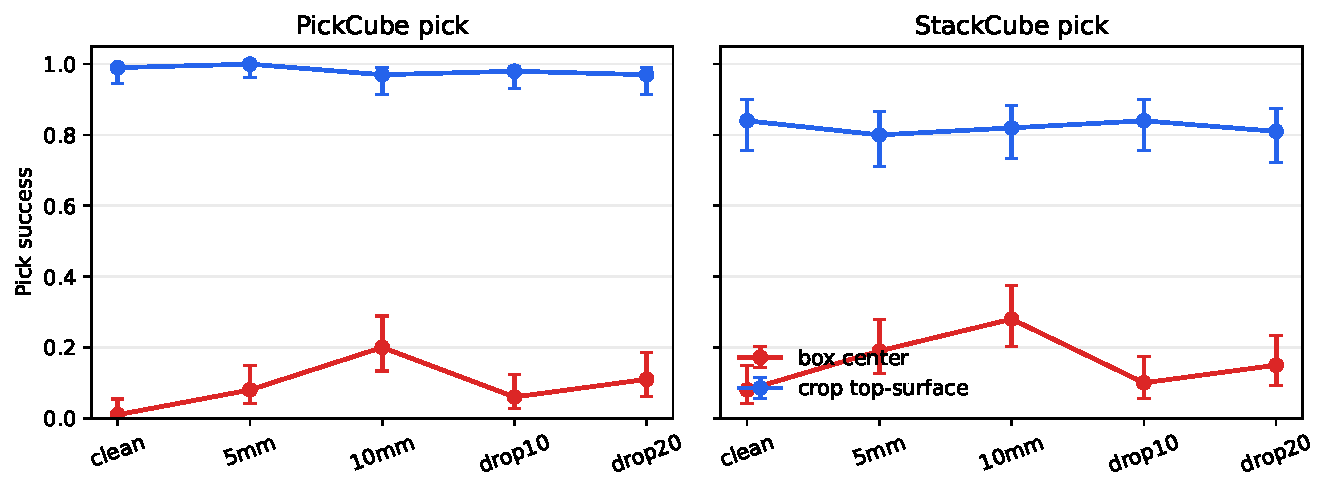
\includegraphics[width=\linewidth]{figures/figure_sensor_stress_pick_success.pdf}
\caption{Pick success under synthetic RGB-D depth perturbations. The
crop-top-surface target remains substantially more executable than the
single-pixel box-center depth source across the tested depth-noise and
dropout levels.}
\label{fig:sensor-stress-pick}
\end{figure}

\begin{figure}[t]
\centering
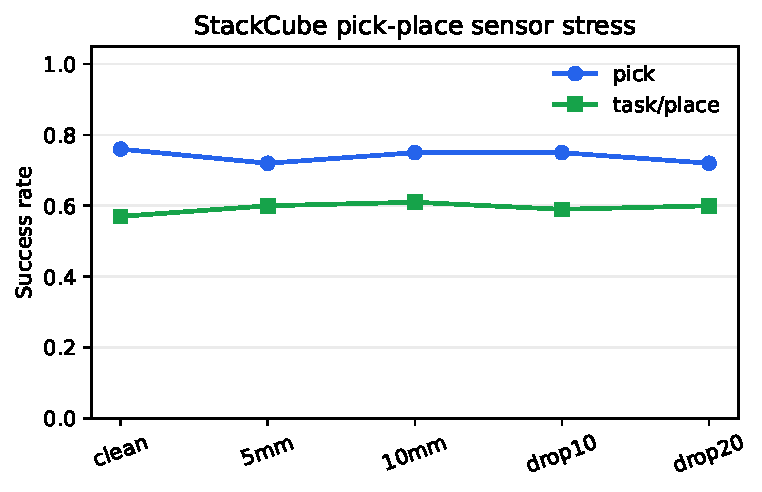
\includegraphics[width=0.85\linewidth]{figures/figure_sensor_stress_task_success.pdf}
\caption{StackCube pick-place sensor stress with crop-top-surface pick targets
and predicted green-cube reference placement. Moderate synthetic depth noise
and dropout do not remove the remaining reference-placement bottleneck.}
\label{fig:sensor-stress-task}
\end{figure}

\section{Discussion}

\subsection{Why Target-Source Quality Deserves Separate Evaluation}

Final task success hides the interface between language-conditioned retrieval
and control. Query-to-Grasp shows that the same detected object can lead to
near-zero or near-oracle execution depending on the selected RGB-D target
source.

This is the main reason for using a diagnostic ladder instead of a single
leaderboard score. A language-conditioned detector can succeed semantically
while producing a crop whose center pixel lies on a depth discontinuity, table
surface, shadowed region, or object edge. Conversely, a simple crop aggregation
heuristic can become highly executable in clean scenes without requiring a
large policy model. By reporting semantic selection, target availability, pick
success, place success, and task success separately, the framework makes the
retrieval-to-execution interface visible.

This taxonomy is not a separate classifier; it is a reporting convention used
to prevent runtime failures, executor mismatch, and target-source failures from
being conflated.

\begin{table}[t]
\centering
\caption{Failure taxonomy used to interpret target-source diagnostics. The
table separates target-source failure, executor mismatch, and
placement/reference failure.}
\label{tab:failure-taxonomy}
\small
\setlength{\tabcolsep}{3pt}
\begin{tabular}{p{0.18\linewidth}p{0.24\linewidth}p{0.20\linewidth}p{0.24\linewidth}}
\toprule
Failure mode & Typical evidence & Affected sources & Diagnostic interpretation \\
\midrule
Target formed but pick fails &
\texttt{target\_available}=1, \texttt{pick\_success}=0 &
PickSingleYCB crop sources &
3D target exists but is not executable by the current primitive \\
\midrule
Oracle succeeds, crop fails &
\texttt{oracle\_object\_pose} far above crop-derived sources &
PickSingleYCB, crop baselines &
Target-source quality, not only controller availability, limits execution \\
\midrule
Oracle also fails &
Oracle pick success near zero or unstable &
LiftPeg and incompatible non-cube settings &
Executor geometry mismatch; not counted as perception-only failure \\
\midrule
Box-center depth weak &
Low pick success despite target availability &
\texttt{box\_center\_depth} &
2D box center is not a reliable 3D action point \\
\midrule
Placement/reference failure &
Pick succeeds but place or task fails &
StackCube predicted-reference rows &
Reference-object association or placement-target precision is the bottleneck \\
\midrule
Sensor-stress sensitivity &
Success or target statistics change under depth noise/dropout &
Sensor-stress rows &
RGB-D degradation perturbs the target-source interface \\
\bottomrule
\end{tabular}
\end{table}


\subsection{Why More Views Are Not Automatically Better}

Additional views can improve recall while also increasing association and
fusion risk. This explains why closed-loop re-observation is treated as a
diagnostic module rather than a guaranteed improvement.

The StackCube results show this tension. Multi-view and closed-loop modes can
increase support and reduce uncertainty, but they can also introduce wrong
object absorption or shift the effective action target. This matters for
systems that use active perception as a default remedy for uncertainty. The
question should not be only whether an extra view reduces a semantic score; it
should be whether the resulting fused target remains accurate enough for
contact-rich execution.

\subsection{Why Scripted Execution Is a Diagnostic Choice}

The scripted executor is not a policy contribution. It fixes the control layer
so that differences in performance can be attributed to target-source quality,
placement-target selection, and geometry.

This design choice is especially important for a diagnostic paper. A learned
policy could compensate for some target errors, fail for unrelated reasons, or
introduce new confounds from training data and architecture. The scripted
controller is intentionally limited, but its limitations are measurable. When
oracle StackCube pick-place reaches 0.880 task success, the controller is shown
to be capable under privileged target sources. When LiftPeg remains at 0.000
even with oracle targets, the controller geometry is exposed as the limiting
factor.

\subsection{Implications for VLM/VLA Robot Systems}

Language and vision models can retrieve plausible targets, but a robot system
still needs a reliable target-source interface before action. Query-to-Grasp
provides a way to audit this interface before adding policy capacity.

This is relevant to VLM/VLA pipelines because language-conditioned action
models often hide perception, grounding, memory, and control inside a single
end-to-end evaluation. The present results suggest that failures should be
decomposed before attributing them to language understanding. In the evaluated
settings, CLIP reranking has no top-1 effect, while centimeter-scale target
errors strongly affect execution. A stronger policy may still help, but it
should be evaluated alongside explicit target-source diagnostics.

\subsection{Sim-to-Real Implications}

The centimeter-level sensitivity results suggest that physical RGB-D systems
should be evaluated for depth noise, calibration error, and crop contamination
before real hardware deployment. The synthetic sensor-stress experiment adds a
first controlled proxy for depth noise and depth dropout, but it remains a
simulation-only diagnostic rather than physical validation.

In physical systems, camera calibration, rolling shutter, depth holes,
reflective surfaces, and object motion can all perturb the target source. The
noisy-oracle curves provide a simulated proxy for how severe such perturbations
can be. They do not replace real-world validation, but they motivate a cautious
deployment path: first measure whether the perception stack can produce stable
3D targets, then test whether a controller can execute them, and only then
interpret full task success.

\section{Limitations and Future Work}

The present study is simulated and does not report physical robot execution.
This is the central limitation of the manuscript. It is acceptable for the
present diagnostic scope because the paper studies controlled
retrieval-to-execution interfaces, but it does not establish hardware
deployment. A physical follow-up should first evaluate RGB-D target-source
stability with real camera intrinsics, depth holes, calibration error, and
lighting variation, and only then test full robot trials.

The controller is scripted and intentionally limited. This choice makes target
sources comparable, but it also excludes object geometries that require side
grasps, wrist rotation, or learned 6-DoF grasp synthesis. LiftPeg demonstrates
this boundary: even an oracle target source cannot make a cube-oriented
top-down primitive grasp a long peg. Future work should connect the same
target-source ladder to AnyGrasp-, Contact-GraspNet-, or policy-based
executors while preserving the diagnostic separation between perception,
target selection, grasp generation, and control.

The executable positive tasks remain cube-heavy. PickSingleYCB provides a
useful non-cube diagnostic because the oracle object pose is partially
executable over 1,600 seeds, but the crop-derived target sources remain weak.
This prevents overclaiming: the current paper can report target-source
sensitivity beyond cube geometry, but it cannot claim broad non-cube
manipulation. A stronger journal extension would add more task-compatible
non-cube objects, evaluate memory targets on matched seeds, and connect the
target-source ladder to a shape-aware 6-DoF grasp generator.

Finally, language and active perception are deliberately simple. The current
reference-object placement bridge uses explicit queries such as ``green
cube'', not robust relation-heavy grounding. Re-observation uses virtual
ManiSkill camera views and a rule-based trigger, so the results should be read
as a diagnostic of this policy rather than a general statement about active
perception. Future work should add relation-aware parsing, real camera motion,
cluttered physical RGB-D captures, calibration-noise sweeps, and real robot-arm
trials with the same artifact-backed reporting discipline used here.

\section{Conclusion}

Query-to-Grasp reframes open-vocabulary RGB-D manipulation as a target-source
diagnostic problem. The results show that 2D retrieval is not enough:
crop-level and memory targets are far more executable than box-center depth,
camera-frame alignment is necessary for multi-view memory, StackCube exposes
reference-object and placement-target limits, and centimeter-level target error
can collapse execution. These diagnostics provide a reproducible basis for
deciding what must be fixed before deploying broader robot policies.

\clearpage
\appendix
\section{Full Sensor-Stress Table}
\label{app:sensor-stress}

The compact sensor-stress table in the main text reports the primary trend.
Table~\ref{tab:sensor-stress} gives the full Wilson-interval diagnostic for
all tested conditions. This table is included for reproducibility and should
be read as a simulation proxy, not as real-world validation.

\begin{table*}[t]
\centering
\caption{Synthetic RGB-D sensor-stress diagnostic. Noise and dropout are applied before 3D target extraction. Values are success rates with Wilson 95\% confidence intervals. This is a simulation proxy, not real-world validation.}
\label{tab:sensor-stress}
\small
\begin{tabular}{llrrrr}
\toprule
Task / source & Condition & $N$ & Target avail. & Pick & Task/raw \\
\midrule
PickCube pick / box center & clean & 100 & 1.000 [0.963,1.000] & 0.010 [0.002,0.054] & 0.020 [0.006,0.070] \\
PickCube pick / box center & depth noise 5 mm & 100 & 1.000 [0.963,1.000] & 0.080 [0.041,0.150] & 0.020 [0.006,0.070] \\
PickCube pick / box center & depth noise 10 mm & 100 & 1.000 [0.963,1.000] & 0.200 [0.133,0.289] & 0.020 [0.006,0.070] \\
PickCube pick / box center & depth dropout 10\% & 100 & 1.000 [0.963,1.000] & 0.060 [0.028,0.125] & 0.020 [0.006,0.070] \\
PickCube pick / box center & depth dropout 20\% & 100 & 1.000 [0.963,1.000] & 0.110 [0.063,0.186] & 0.020 [0.006,0.070] \\
\midrule
PickCube pick / crop top-surface & clean & 100 & 1.000 [0.963,1.000] & 0.990 [0.946,0.998] & 0.010 [0.002,0.054] \\
PickCube pick / crop top-surface & depth noise 5 mm & 100 & 1.000 [0.963,1.000] & 1.000 [0.963,1.000] & 0.030 [0.010,0.085] \\
PickCube pick / crop top-surface & depth noise 10 mm & 100 & 1.000 [0.963,1.000] & 0.970 [0.915,0.990] & 0.010 [0.002,0.054] \\
PickCube pick / crop top-surface & depth dropout 10\% & 100 & 1.000 [0.963,1.000] & 0.980 [0.930,0.994] & 0.010 [0.002,0.054] \\
PickCube pick / crop top-surface & depth dropout 20\% & 100 & 1.000 [0.963,1.000] & 0.970 [0.915,0.990] & 0.010 [0.002,0.054] \\
\midrule
StackCube pick / box center & clean & 100 & 1.000 [0.963,1.000] & 0.080 [0.041,0.150] & 0.000 [0.000,0.037] \\
StackCube pick / box center & depth noise 5 mm & 100 & 1.000 [0.963,1.000] & 0.190 [0.125,0.278] & 0.000 [0.000,0.037] \\
StackCube pick / box center & depth noise 10 mm & 100 & 1.000 [0.963,1.000] & 0.280 [0.201,0.375] & 0.000 [0.000,0.037] \\
StackCube pick / box center & depth dropout 10\% & 100 & 1.000 [0.963,1.000] & 0.100 [0.055,0.174] & 0.000 [0.000,0.037] \\
StackCube pick / box center & depth dropout 20\% & 100 & 1.000 [0.963,1.000] & 0.150 [0.093,0.233] & 0.000 [0.000,0.037] \\
\midrule
StackCube pick / crop top-surface & clean & 100 & 1.000 [0.963,1.000] & 0.840 [0.756,0.899] & 0.000 [0.000,0.037] \\
StackCube pick / crop top-surface & depth noise 5 mm & 100 & 1.000 [0.963,1.000] & 0.800 [0.711,0.867] & 0.000 [0.000,0.037] \\
StackCube pick / crop top-surface & depth noise 10 mm & 100 & 1.000 [0.963,1.000] & 0.820 [0.733,0.883] & 0.000 [0.000,0.037] \\
StackCube pick / crop top-surface & depth dropout 10\% & 100 & 1.000 [0.963,1.000] & 0.840 [0.756,0.899] & 0.000 [0.000,0.037] \\
StackCube pick / crop top-surface & depth dropout 20\% & 100 & 1.000 [0.963,1.000] & 0.810 [0.722,0.875] & 0.000 [0.000,0.037] \\
\midrule
StackCube pick-place / crop top-surface & clean & 100 & 1.000 [0.963,1.000] & 0.760 [0.668,0.833] & 0.570 [0.472,0.663] \\
StackCube pick-place / crop top-surface & depth noise 5 mm & 100 & 1.000 [0.963,1.000] & 0.720 [0.625,0.799] & 0.600 [0.502,0.691] \\
StackCube pick-place / crop top-surface & depth noise 10 mm & 100 & 1.000 [0.963,1.000] & 0.750 [0.657,0.825] & 0.610 [0.512,0.700] \\
StackCube pick-place / crop top-surface & depth dropout 10\% & 100 & 1.000 [0.963,1.000] & 0.750 [0.657,0.825] & 0.590 [0.492,0.681] \\
StackCube pick-place / crop top-surface & depth dropout 20\% & 100 & 1.000 [0.963,1.000] & 0.720 [0.625,0.799] & 0.600 [0.502,0.691] \\
\bottomrule
\end{tabular}
\end{table*}

\clearpage

\section*{Data Availability}

The code repository for Query-to-Grasp is available at
\url{https://github.com/KleinChen42/Query-to-Grasp}. The submitted artifact
package contains benchmark summaries, per-run rows, table-generation scripts,
figure-generation scripts, and lightweight inventory reports used to reproduce
the reported tables and figures.

\section*{Declaration of Generative AI and AI-Assisted Technologies}

During manuscript preparation, AI-assisted tools were used for drafting,
editing, code assistance, and experiment-planning support. The author reviewed,
edited, and takes responsibility for all scientific claims, results, code, and
final manuscript content.

\section*{Funding}

No funding was declared for this manuscript.

\section*{Declaration of Competing Interest}

The author declares no known competing financial interests or personal
relationships that could have appeared to influence the work reported in this
paper.

\section*{CRediT Author Statement}

Zhuo Chen: Conceptualization, Methodology, Software, Validation,
Investigation, Data Curation, Writing - Original Draft, Writing - Review and
Editing, Visualization.

\bibliographystyle{elsarticle-num}
\bibliography{references}

\end{document}
